\documentclass{beamer}
\usepackage[utf8]{inputenc}

\usetheme{Madrid}
\usecolortheme{default}
\usepackage{amsmath,amssymb,amsfonts,amsthm}
\usepackage{txfonts}
\usepackage{tkz-euclide}
\usepackage{listings}
\usepackage{adjustbox}
\usepackage{array}
\usepackage{tabularx}
\usepackage{gvv}
\usepackage{lmodern}
\usepackage{circuitikz}
\usepackage{tikz}
\usepackage{graphicx}

\setbeamertemplate{page number in head/foot}[totalframenumber]

\usepackage{tcolorbox}
\tcbuselibrary{minted,breakable,xparse,skins}



\definecolor{bg}{gray}{0.95}
\DeclareTCBListing{mintedbox}{O{}m!O{}}{%
  breakable=true,
  listing engine=minted,
  listing only,
  minted language=#2,
  minted style=default,
  minted options={%
    linenos,
    gobble=0,
    breaklines=true,
    breakafter=,,
    fontsize=\small,
    numbersep=8pt,
    #1},
  boxsep=0pt,
  left skip=0pt,
  right skip=0pt,
  left=25pt,
  right=0pt,
  top=3pt,
  bottom=3pt,
  arc=5pt,
  leftrule=0pt,
  rightrule=0pt,
  bottomrule=2pt,
  toprule=2pt,
  colback=bg,
  colframe=orange!70,
  enhanced,
  overlay={%
    \begin{tcbclipinterior}
    \fill[orange!20!white] (frame.south west) rectangle ([xshift=20pt]frame.north west);
    \end{tcbclipinterior}},
  #3,
}
\lstset{
    language=C,
    basicstyle=\ttfamily\small,
    keywordstyle=\color{blue},
    stringstyle=\color{orange},
    commentstyle=\color{green!60!black},
    numbers=left,
    numberstyle=\tiny\color{gray},
    breaklines=true,
    showstringspaces=false,
}
%------------------------------------------------------------
%This block of code defines the information to appear in the
%Title page
\title %optional
{1.4.25}
\date{August 30,2025}
%\subtitle{A short story}

\author % (optional)
{Anshu kumar ram-EE25BTECH11009}



\begin{document}


\frame{\titlepage}
% ---------------- Question ----------------
\begin{frame}{Question}
\textbf{Find the position vector of a point $\vec{R}$ which divides the line joining two points $\vec{P}$ and $\vec{Q}$ whose position vectors are $2\vec{a} + \vec{b}$ and $\vec{a} - 3\vec{b}$ externally in the ratio $1:2$.}
\end{frame}

% ---------------- Solution Step 1 ----------------
\begin{frame}{Solution Step 1}
\textbf{Step 1: Express $\vec{P}, \vec{Q}$ in terms of $\vec{a}, \vec{b}$}  

\begin{align}
\vec{P} &= 2\vec{a} + \vec{b}, \label{eq:P}\\
\vec{Q} &= \vec{a} - 3\vec{b}. \label{eq:Q}
\end{align}

Stacking $\vec{P}, \vec{Q}$ into a matrix:
\begin{align}
\myvec{\vec{P} & \vec{Q}}
= \myvec{\vec{a} & \vec{b}}
  \myvec{2 & 1 \\ 1 & -3}
\label{eq:PQ-matrix}
\end{align}
\end{frame}

% ---------------- Solution Step 2 ----------------
\begin{frame}{Solution Step 2}
\textbf{Step 2: Section formula for external division}  

For ratio $1:2$,  
\begin{align}
\vec{R} &= \frac{1\vec{Q} - 2\vec{P}}{1-2} \label{eq:section}
\end{align}

In matrix form:
\begin{align}
\vec{R} &= \frac{1}{-1}\,\myvec{\vec{P} & \vec{Q}}\myvec{-2 \\ 1}
\label{eq:R-matrix}
\end{align}
\end{frame}

% ---------------- Solution Step 3 ----------------
\begin{frame}{Solution Step 3}
\textbf{Step 3: Substitute $\vec{P}, \vec{Q}$ in terms of $\vec{a}, \vec{b}$}  

\begin{align}
\vec{R}
&= \frac{1}{-1}\,
   \myvec{\vec{a} & \vec{b}}
   \myvec{2 & 1 \\ 1 & -3}
   \myvec{-2 \\ 1} \label{eq:R-sub1} \\[6pt]
&= \frac{1}{-1}\,
   \myvec{\vec{a} & \vec{b}}
   \myvec{-3 \\ -5} \label{eq:R-sub2} \\[6pt]
&= \myvec{\vec{a} & \vec{b}}
   \myvec{3 \\ 5} \label{eq:R-final}
\end{align}

\[
\boxed{\vec{R} = 3\vec{a} + 5\vec{b}}
\]
\end{frame}

% ---------% ---------------- C Code ----------------
\begin{frame}[fragile]{C Code: section() Function}
\begin{lstlisting}[style=CStyle]
void section(double* P, double* Q, double* R, int m) {
    for (int i = 0; i < m; i++) {
        R[i] = (Q[i] - 2 * P[i]) / (1 - 2);
    }
}
\end{lstlisting}
\end{frame}

\begin{frame}[fragile]{C Code: line\_gen() Function}
\begin{lstlisting}[style=CStyle]
void line_gen(double* X, double* Y, const double* A, const double* B, int n, int m) {
    double temp[2];
    for (int i = 0; i < 2; i++) {
        temp[i] = (B[i] - A[i]) / (double)n;
    }
    for (int i = 0; i <= n; i++) {
        X[i] = A[0] + temp[0] * i;
        Y[i] = A[1] + temp[1] * i;
    }
}
\end{lstlisting}
\end{frame}

% ---------------- Python with C Integration ----------------
\begin{frame}[fragile]{Python + C: Load Library}
\begin{lstlisting}[style=PyStyle]
import ctypes
import numpy as np
import matplotlib.pyplot as plt

handc = ctypes.CDLL("./func.so")

# section function
handc.section.argtypes = [
    ctypes.POINTER(ctypes.c_double),
    ctypes.POINTER(ctypes.c_double),
    ctypes.POINTER(ctypes.c_double),
    ctypes.c_int
]
handc.section.restype = None

# line_gen function
handc.line_gen.argtypes = [
    ctypes.POINTER(ctypes.c_double),
    ctypes.POINTER(ctypes.c_double),
    ctypes.POINTER(ctypes.c_double),
    ctypes.POINTER(ctypes.c_double),
    ctypes.c_int,
    ctypes.c_int
]
handc.line_gen.restype = None
\end{lstlisting}
\end{frame}

\begin{frame}[fragile]{Python + C: Compute \& Plot}
\begin{lstlisting}[style=PyStyle]
m = 2
a = np.array([1,0], dtype=np.float64)
b = np.array([0,1], dtype=np.float64)
P = 2*a + b
Q = a - 3*b
R = np.zeros(m, dtype=np.float64)

handc.section(P.ctypes.data_as(ctypes.POINTER(ctypes.c_double)),
              Q.ctypes.data_as(ctypes.POINTER(ctypes.c_double)),
              R.ctypes.data_as(ctypes.POINTER(ctypes.c_double)),
              m)

n = 20
X_l = np.zeros(n, dtype=np.float64)
Y_l = np.zeros(n, dtype=np.float64)
handc.line_gen(X_l.ctypes.data_as(ctypes.POINTER(ctypes.c_double)),
               Y_l.ctypes.data_as(ctypes.POINTER(ctypes.c_double)),
               Q.ctypes.data_as(ctypes.POINTER(ctypes.c_double)),
               R.ctypes.data_as(ctypes.POINTER(ctypes.c_double)),
               n, m)

plt.plot(X_l, Y_l, "g--", label="Line PQ")
plt.scatter(P[0], P[1], color="blue", s=50)
plt.scatter(Q[0], Q[1], color="green", s=50)
plt.scatter(R[0], R[1], color="red", s=50, label="R")
plt.show()
\end{lstlisting}
\end{frame}

% ---------------- Pure Python ----------------
\begin{frame}[fragile]{Pure Python: Functions \& Setup}
\begin{lstlisting}[style=PyStyle]
import sys
sys.path.insert(0, '/home/anshu-ram/matgeo/codes/CoordGeo')
import numpy as np
import matplotlib.pyplot as plt

from line.funcs import *
from triangle.funcs import *
from conics.funcs import circ_gen

def section_point(P, Q, m, n, external=True):
    if external:
        return (m*Q - n*P)/(m-n)
    else:
        return (m*Q + n*P)/(m+n)
\end{lstlisting}
\end{frame}

\begin{frame}[fragile]{Pure Python: Compute \& Plot}
\begin{lstlisting}[style=PyStyle]
a = np.array([1,0]).reshape(-1,1)
b = np.array([0,1]).reshape(-1,1)
P = 2*a + b
Q = a - 3*b
R = section_point(P, Q, 1, 2, external=True)

x_PQ = line_gen_num(P, Q, 20)
x_PR = line_gen_num(P, R, 20)
x_QR = line_gen_num(Q, R, 20)

plt.plot(x_PQ[0,:], x_PQ[1,:], "g--", label="Line PQ")
plt.plot(x_PR[0,:], x_PR[1,:], "r--", label="Line PR")
plt.plot(x_QR[0,:], x_QR[1,:], "b--", label="Line QR")
tri_coords = np.hstack((P,Q,R))
plt.scatter(tri_coords[0,:], tri_coords[1,:])
plt.show()
\end{lstlisting}
\end{frame}
\begin{frame}{Plot}
    \centering
    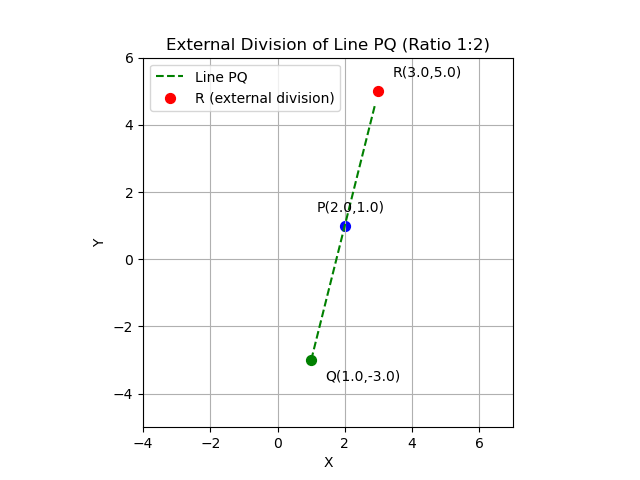
\includegraphics[width=\columnwidth, height=0.8\textheight, keepaspectratio]{figs/section_graph.png}     
\end{frame}


\end{document}
